\chapter{Handling Millions of Atomic Structures} \label{chap:mpdd}

\acknowledge{
This chapter adapts parts of a manuscript draft planned for publication before dissertation submission, co-authored with Ricardo Amaral, Jonathan W. Siegel, and Zi-Kui Liu. All of included text was written by Adam M. Krajewski. Described software has been developed by Adam M. Krajewski since 2020 with assistance from Jonathan W. Siegel and Ricardo Amaral. Zi-Kui Liu provided edits and guidance. It also adapts excerpt written by Adam M. Krajewski for \citet{Evans2024DevelopmentsExchange} reproduced from Digital Discovery journal under CC BY 3.0 license. 
}


\section{Introduction} \label{mpdd:sec:background}

Traditionally, the field of materials science deals with highly complex data, in terms of both input and output descriptions, acquired through laborious experiments in the laboratories, such as mechanical or electrochemical tests performed according to professional standards, or expensive computations on supercomputer clusters, including ones based on the density functional theory (DFT)~\cite{Kohn1996DensityStructure} or finite element method (FEM)~\cite{Liu2022EightyFuture}. Because of this high-cost aspect, the number of datapoints being generated is usually very limited, especially after raw data is fitted into models, and disseminated through reports and scientific publications as typeset tables, text, or figures, which are then carefully interpreted by other researchers.

In the last few decades, however, the community is becoming increasingly engages in large-scale efforts to construct large collections of data points, especially after endorsement and special funding was provided by the Materials Genome Initiative in 2011 \cite{SubcommitteeontheMaterialsGenomeInitiative2021MaterialsPlan, Agren2023CALPHADAnniversary, Olson2023GenomicDynamics}. It significantly accelerated many efforts to combine materials-specific scientific literature sources into a homogeneous structure were attempted, with perhaps the most successful being the \texttt{Pauling File} developed since 1995 with as of 2024, was built with 1000 years of full-time academic effort \cite{Blokhin2018TheGenome} and underlies several databases, including ASM Phase Diagram Database \cite{ASMInternational} and Materials Platform for Data Science (MPDS) \cite{Blokhin2018TheGenome}. Furthermore, a number of computational databases listed later in Section~\ref{mpdd:ssec:dataset}, were also created and in some cases grew beyond one million entries.

With the rise of such large-scale databases, it becomes critical to be able to efficiently operate on them and utilize them, as even seemingly fast calculations of $1s$ grow to over 8 weeks when performed 5 million times. Furthermore, this scale is likely to sharply increase in the near future due to a large volume of data coming from machine learning (ML) studies with, even if filtered out, will likely accelerate search efforts using more traditional computation by constantly providing guidance.


\section{The Material-Property-Descriptor Database} \label{mpdd:sec:mpdd}

\subsection{Motivation} \label{mpdd:ssec:motivation}

The Material-Property-Descriptor Database (MPDD) is an extensive (4.5M+) database of \emph{ab initio} relaxations of 3D crystal structures,  combined with an infrastructure of tools allowing efficient descriptor calculation (featurization), as well as the deployment of ML models like \texttt{SIPFENN} \cite{Krajewski2024EfficientStructures} described in Chapter \ref{chap:sipfenn}, and other developed by the community including \texttt{ALIGNN} \cite{Choudhary2021AtomisticPredictions} and \texttt{CHGNet} \cite{Deng2023CHGNetModelling}.

The most critical motivation behind MPDD is the retention of intermediate modeling data (atomistic features), including structure-informed descriptors described in Chapter \ref{chap:pysipfenn}, which typically cost orders of magnitude more computational time than any of the other steps performed during ML model deployment~\cite{Krajewski2022ExtensibleNetworks}. Thus, many ML models can be run at a small fraction of the original cost if the same descriptor (or, more commonly, a subset chosen through feature selection) is used. This benefit applies regardless of whether a model is just another iteration, e.g., fine-tuned to a specific class of materials like perovskites, or an entirely new model for a different property. Thanks to this, machine learning researchers can effortlessly take advantage of MPDD to deploy numerous ML models directly to the community without needing to construct individual deployment targets, which are typically both much smaller and redundant relative to existing datasets.

Furthermore, MPDD's access to stored atomic structures and associated metadata has been shown to be useful, for instance, in the fully data-driven prediction of atomic structures (validated with DFT and experiments). It, for instance allowed quick identification of unknown structures in Nd-Bi~\cite{Im2022ThermodynamicModeling} and Al-Fe~\cite{Shang2021FormingJoints} systems, what is discussed in more detail in Chapter \ref{chap:crystall}.


\subsection{Dataset} \label{mpdd:ssec:dataset}

To act as both the starting point for both (a) generative design of new datapoints and (b) deployment target for forward methods, a large collection of atomic structures has been collected and homogenized into the \texttt{MPDD}. It contained \textit{DFT-based datasets} including OQMD \cite{Saal2013MaterialsOQMD, Kirklin2015TheEnergies, Shen2022ReflectionsOQMD}, AFLOW \cite{Curtarolo2013AFLOW:Discovery, Toher2018TheDiscovery}, Materials Project \cite{Jain2013Commentary:Innovation}, NIST-JARVIS \cite{Choudhary2020TheDesign}, Alexandria \cite{Schmidt2022AFunctionals}, CAMD \cite{Ye2022NovelAgents}, GNoME \cite{Merchant2023ScalingDiscovery}, \textit{in-house DFT-based datasets} including phonon calculations created with DFTTK \cite{Wang2021DFTTK:Calculations}, as well as hundreds of thousands of experimentally observed entries from Crystallography Open Database (COD) \cite{Grazulis2009CrystallographyStructures, Grazulis2012CrystallographyCollaboration, Grazulis2019CrystallographyPerspectives}. As shown in Figure~\ref{mpdd:fig:dataset}, the collected dataset does not exhibit a bias towards any particular chemical element, but rather it covers tens of different elements almost uniformly.

\begin{figure}[H]
    \centering
    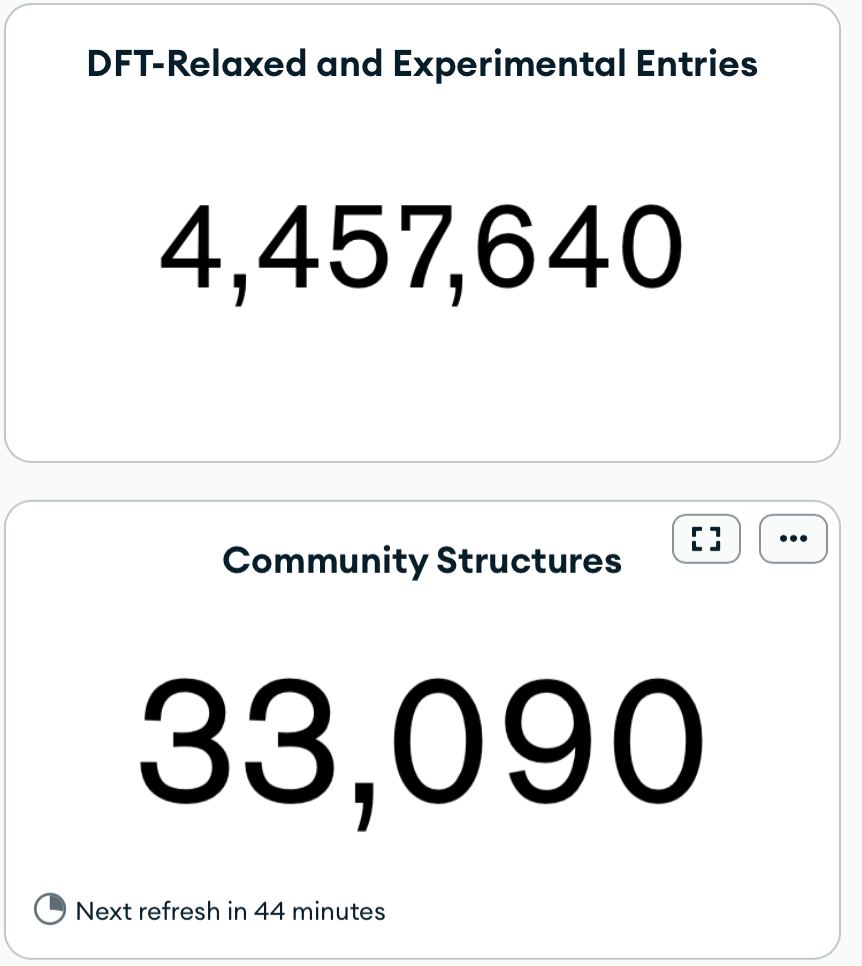
\includegraphics[width=0.4\textwidth]{mpdd/Screenshot 2024-05-05 at 11.54.32.png}
    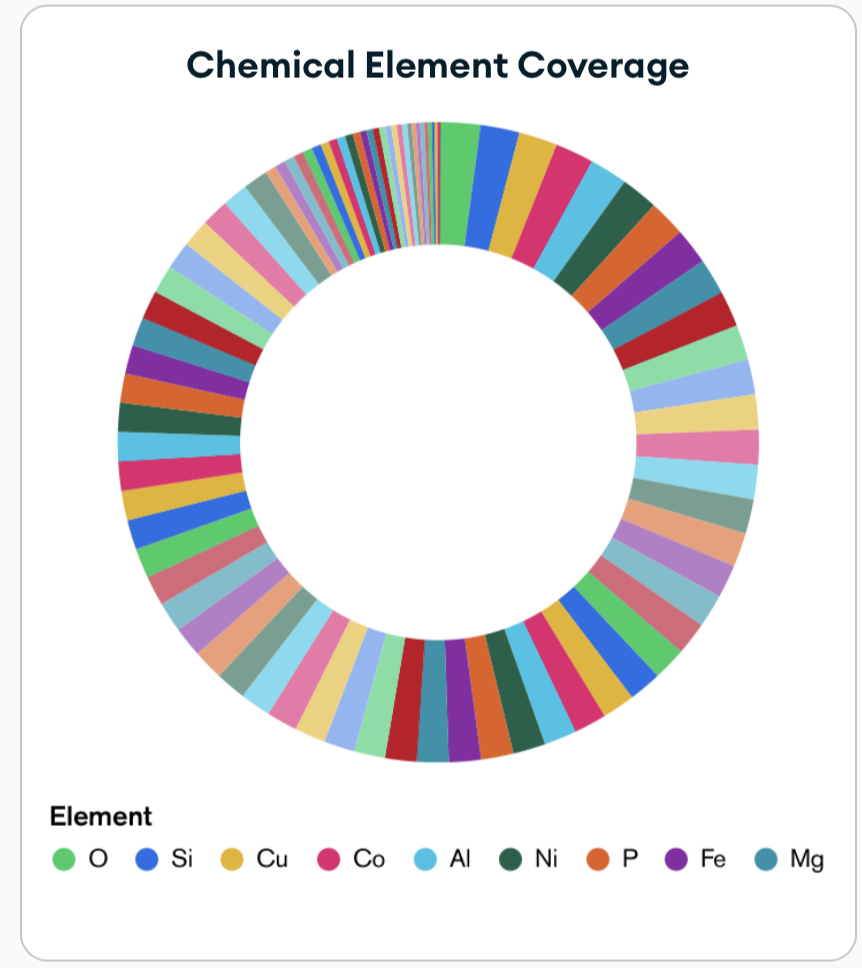
\includegraphics[width=0.4\textwidth]{mpdd/Screenshot 2024-05-05 at 11.54.47.png}
    \caption{Key statistics over MPDD dataset as of April 2024 demonstrating (1) extent of the dataset and (2) high diversity of chemical space coverage over all elements.}
    \label{mpdd:fig:dataset}
\end{figure}

Notably, for the sake of completeness, a substantial effort was made to cover \emph{all 118 elements} by specifically collecting recent experimental observations and DFT-based lattice stability calculations of uncommon elements from several sources. These included
Es, Cf, Cm, Bk based on \citet{2006TheElements}, Lr, Rf, Db, Sg, Bh, Hs, Mt, Ds, Rg based on \citet{Gyanchandani2011PhysicalMetals}, Cn based on \citet{Atta-Fynn2015DensityElements}, Fl based on \citet{MaizHadjAhmed2017RevisitingFlerovium}, Nh based on \citet{Atarah2020FirstNihonium}, Cn, Fl, Lv, Mc, Nh, Og, Ts based on \citet{Trombach2019ExploringTheory}, Fr based on \citet{Koufos2013ElectronicFrancium}, and At based on \citet{Hermann2013CondensedMetallic}, to cover 115 elements. The last 3 (Fm, Md, No), best to author's knowledge, were not yet experimentally measured nor calculated with DFT-based methods, but were approximated based on rationale in \citet{2006TheElements}.


\subsection{Infrastructure} \label{mpdd:ssec:infrastructure}

The designed infrastructure of \texttt{MPDD}, built on top of a \texttt{MongoDB} database framework, is focused on independent methods operating on each datapoint with has (1) a definition of material, (2) descriptor set, and (3) property set, in a way such that one part of the data is augmented by another, as depicted in Figure~\ref{mpdd:fig:core}. This is typically accomplished by using special \texttt{MongoDB} indexes which enable to effectively present the data to a given method as a collection of either of the three, e.g., to select all materials fulfilling requirements) or lack thereof, e.g., to operate on a small subset of incomplete newly inserted data for which a task needs to be run.

\begin{figure}[H]
    \centering
    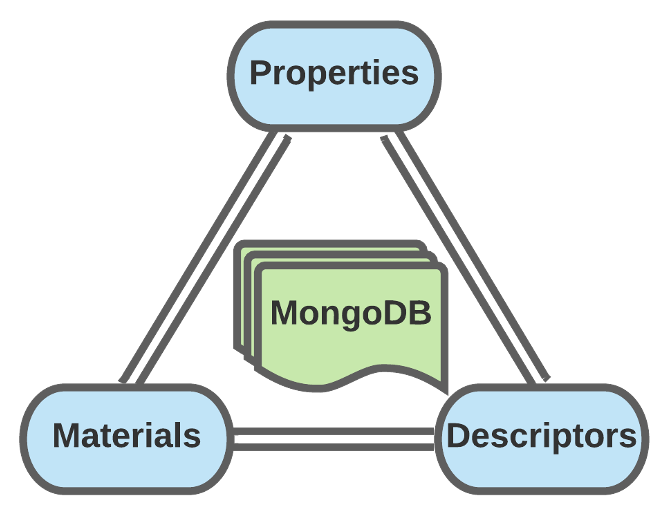
\includegraphics[width=0.4\textwidth]{mpdd/MPDD_CoreTriplet.png}
    \caption{Three entities at the core of MPDD treated as "first class citizens" interacting with each other. Going counter-clockwise \emph{Materials} cover our past sampling of the problem domain, \emph{Descriptors} cover our understanding of it, and \emph{Properties} determine utility. Going clockwise desired \emph{Properties} guide analysis leading to understanding encoded in \emph{Descriptors}, which inform us of unexplored regions of problem domain in their individual contexts.}
    \label{mpdd:fig:core}
\end{figure}

When filled with a large dataset described in Section~\ref{mpdd:ssec:dataset} and combined with generative models extending it (see Chapter~\ref{chap:crystall}), such ecosystem becomes cyclic in nature and thanks to built-in automations can continuously grow, as shown schematically in Figure~\ref{mpdd:fig:schematic}. At the same time, thanks to its decentralized nature, it can be highly parallelized across many devices, ranging from a slow single-board computer to scalable high performance computing (HPC) cluster allocations, enabling handling of variable workloads.


\begin{figure}[H]
    \centering
    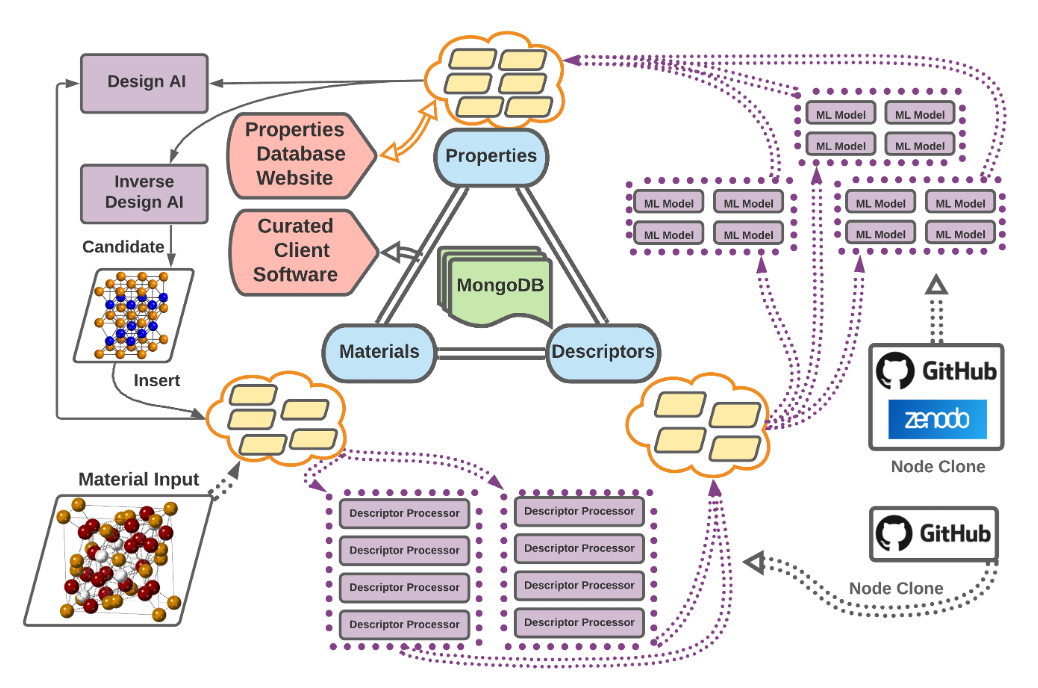
\includegraphics[width=0.9\textwidth]{mpdd/Picture1.png}
    \caption{Main schematic of the MPDD Database infrastructure.}
    \label{mpdd:fig:schematic}
\end{figure}





\section{Open Databases Integration for Materials Design (OPTIMADE) API of MPDD} \label{mpdd:sec:optimade}

\texttt{OPTIMADE} or the Open Databases Integration for Materials Design consortium has been established to make materials databases interoperable by developing a specification for a common REST API \cite{Evans2024DevelopmentsExchange}. That way, databases can remain independently maintained and tuned to specific needs, like ab initio data or ML data, while at the same time reporting on the contained knowledge so that redundant calculations are not performed and the efficiency of the materials informatics community at large is dramatically improved.

MPDD has a stable \texttt{OPTIMADE} API that serves the entire core MPDD dataset, fully implementing \texttt{v1.1.0} of the OPTIMADE standard, as of April 2024, through a cloud server based on \texttt{optimade-python-tools} \cite{Evans2021}.
Making the MPDD available via OPTIMADE was initially challenging, as MPDD stores and exchanges data in a way that prioritises high throughput and low storage requirements, including binary data, making it difficult or slow to make MPDD queryable as an OPTIMADE API on-the-fly.
However, issues have been resolved by establishing a self-updating mirror of the dataset where structures are made OPTIMADE-compliant during transfer, which can occur within the same virtual machine or other integrated computing environment. Most of the MPDD-specific data is available under the \texttt{mpdd} namespace of \texttt{OPTIMADE}, including dictionaries of metadata (e.g., \texttt{\_mpdd\_atomicvolume}), properties (e.g., \texttt{\_mpdd\_formationenergy\_sipfenn\_krajewski2020\_lightmodel}), and descriptors (e.g., \texttt{\_mpdd\_descriptors.KS2022}), described earlier in this chapter.

The base URL is available at:

\hspace{24pt} \href{https://optimade.mpdd.org}{https://optimade.mpdd.org}

and one can see a sample dataset response by following the \texttt{structures} endpoint at:

\hspace{24pt} \href{https://optimade.mpdd.org/v1/structures}{https://optimade.mpdd.org/v1/structures}


\section{MPDD-eXchange} \label{mpdd:sec:mpddx}

In addition to the \texttt{OPTIMADE} API serving as the main endpoint for the end-users, \texttt{MPDD} has recently been extended through an experimental platform availale at \href{https://contrib.mpdd.org}{contrib.mpdd.org} based on GitHub automations to facilitate data exchange; thus, called \texttt{MPDD-eXchange} or \texttt{MPDD-X}. The main exchange, where the user uploads their data, which gets validated and ingested into the data ecosystem enriching the \texttt{MPDD}; while the user gets presented with machine learning predictions associated with it and gets persistent credit associated with their account. 

From the user-perspective all work is being performed entirely within GitHub Issues of the \texttt{MPDD-X} repository, enabling anyone with a free account to start it, as shown in Figure~\ref{mpdd:fig:mpddx1}. 

\begin{figure}[H]
    \centering
    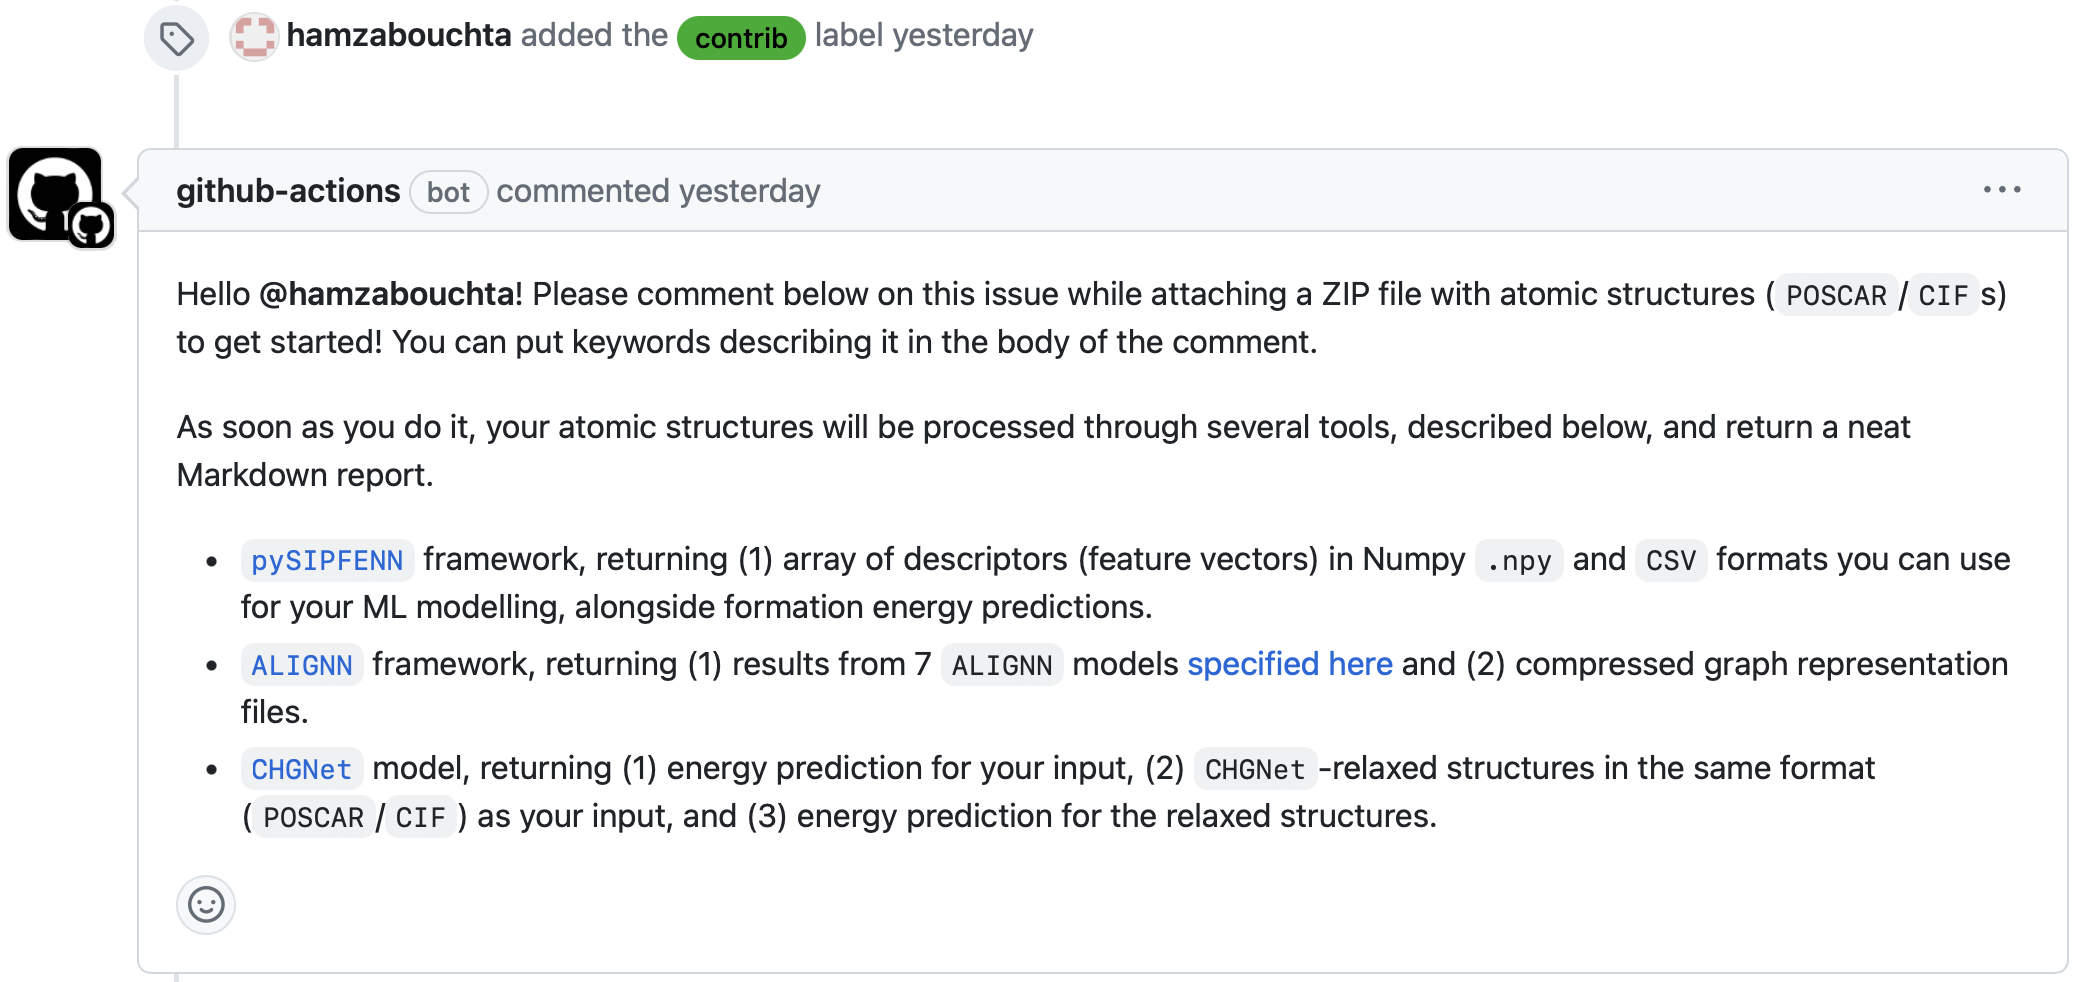
\includegraphics[width=0.7\textwidth]{mpdd/mpddx1.png}
    \caption{Printout of the greeting message on issues opened with auto-assigned \texttt{contrib} label instructing user how to send a contribution and what models will be run.}
    \label{mpdd:fig:mpddx1}
\end{figure}

Once the user opens an Issue, they only need to provide a ZIP file containing either \texttt{CIF} \cite{Hall1991TheCrystallography} or \texttt{POSCAR} \cite{VASPPOSCAR} files, commonly used in the community, what can be done by simply dragging a file into the comment. Momentarily after the ZIP file is posted, an automated action will process it, informing user of the progress, as shown in the example in Figure~\ref{mpdd:fig:mpddx2}.

\begin{figure}[H]
    \centering
    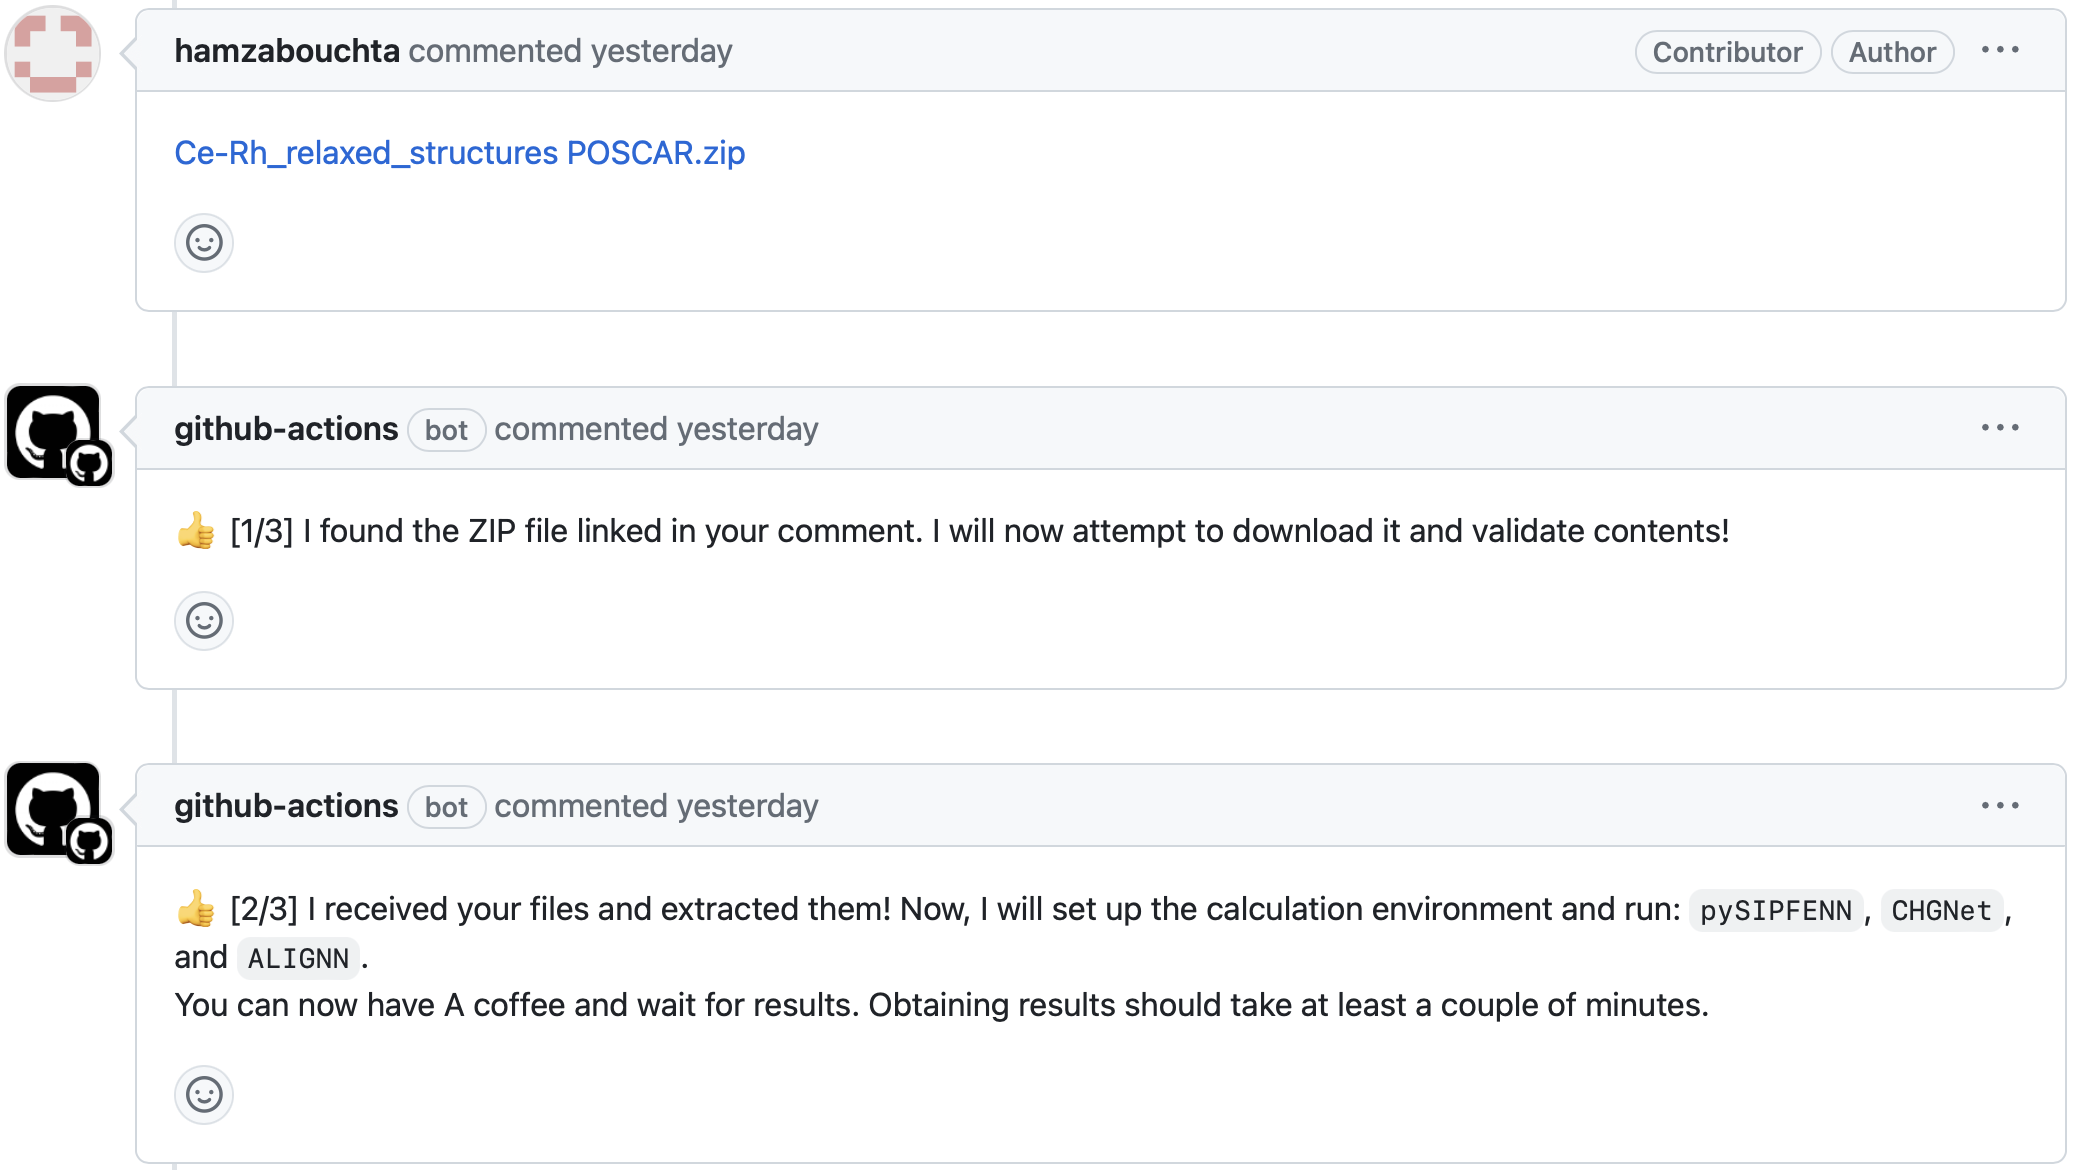
\includegraphics[width=0.8\textwidth]{mpdd/mpddx2.png}
    \caption{Printout of the intermediate messages informing that validation checks are passing, if the user sent a properly formatted CIF or POSCAR files in a ZIP file. Otherwise (not depicted) messages would provide feedback on errors.}
    \label{mpdd:fig:mpddx2}
\end{figure}

Then, typically after 5 to 20 minutes, depending on the task complexity and server load, user gets presented with, as shown in Figure~\ref{mpdd:fig:mpddx3}, (1) a result table with outputs of several literature models, as well as, (2) a persistent identifier which can be used to reference both the results and details of how they were obtained.

\begin{figure}[H]
    \centering
    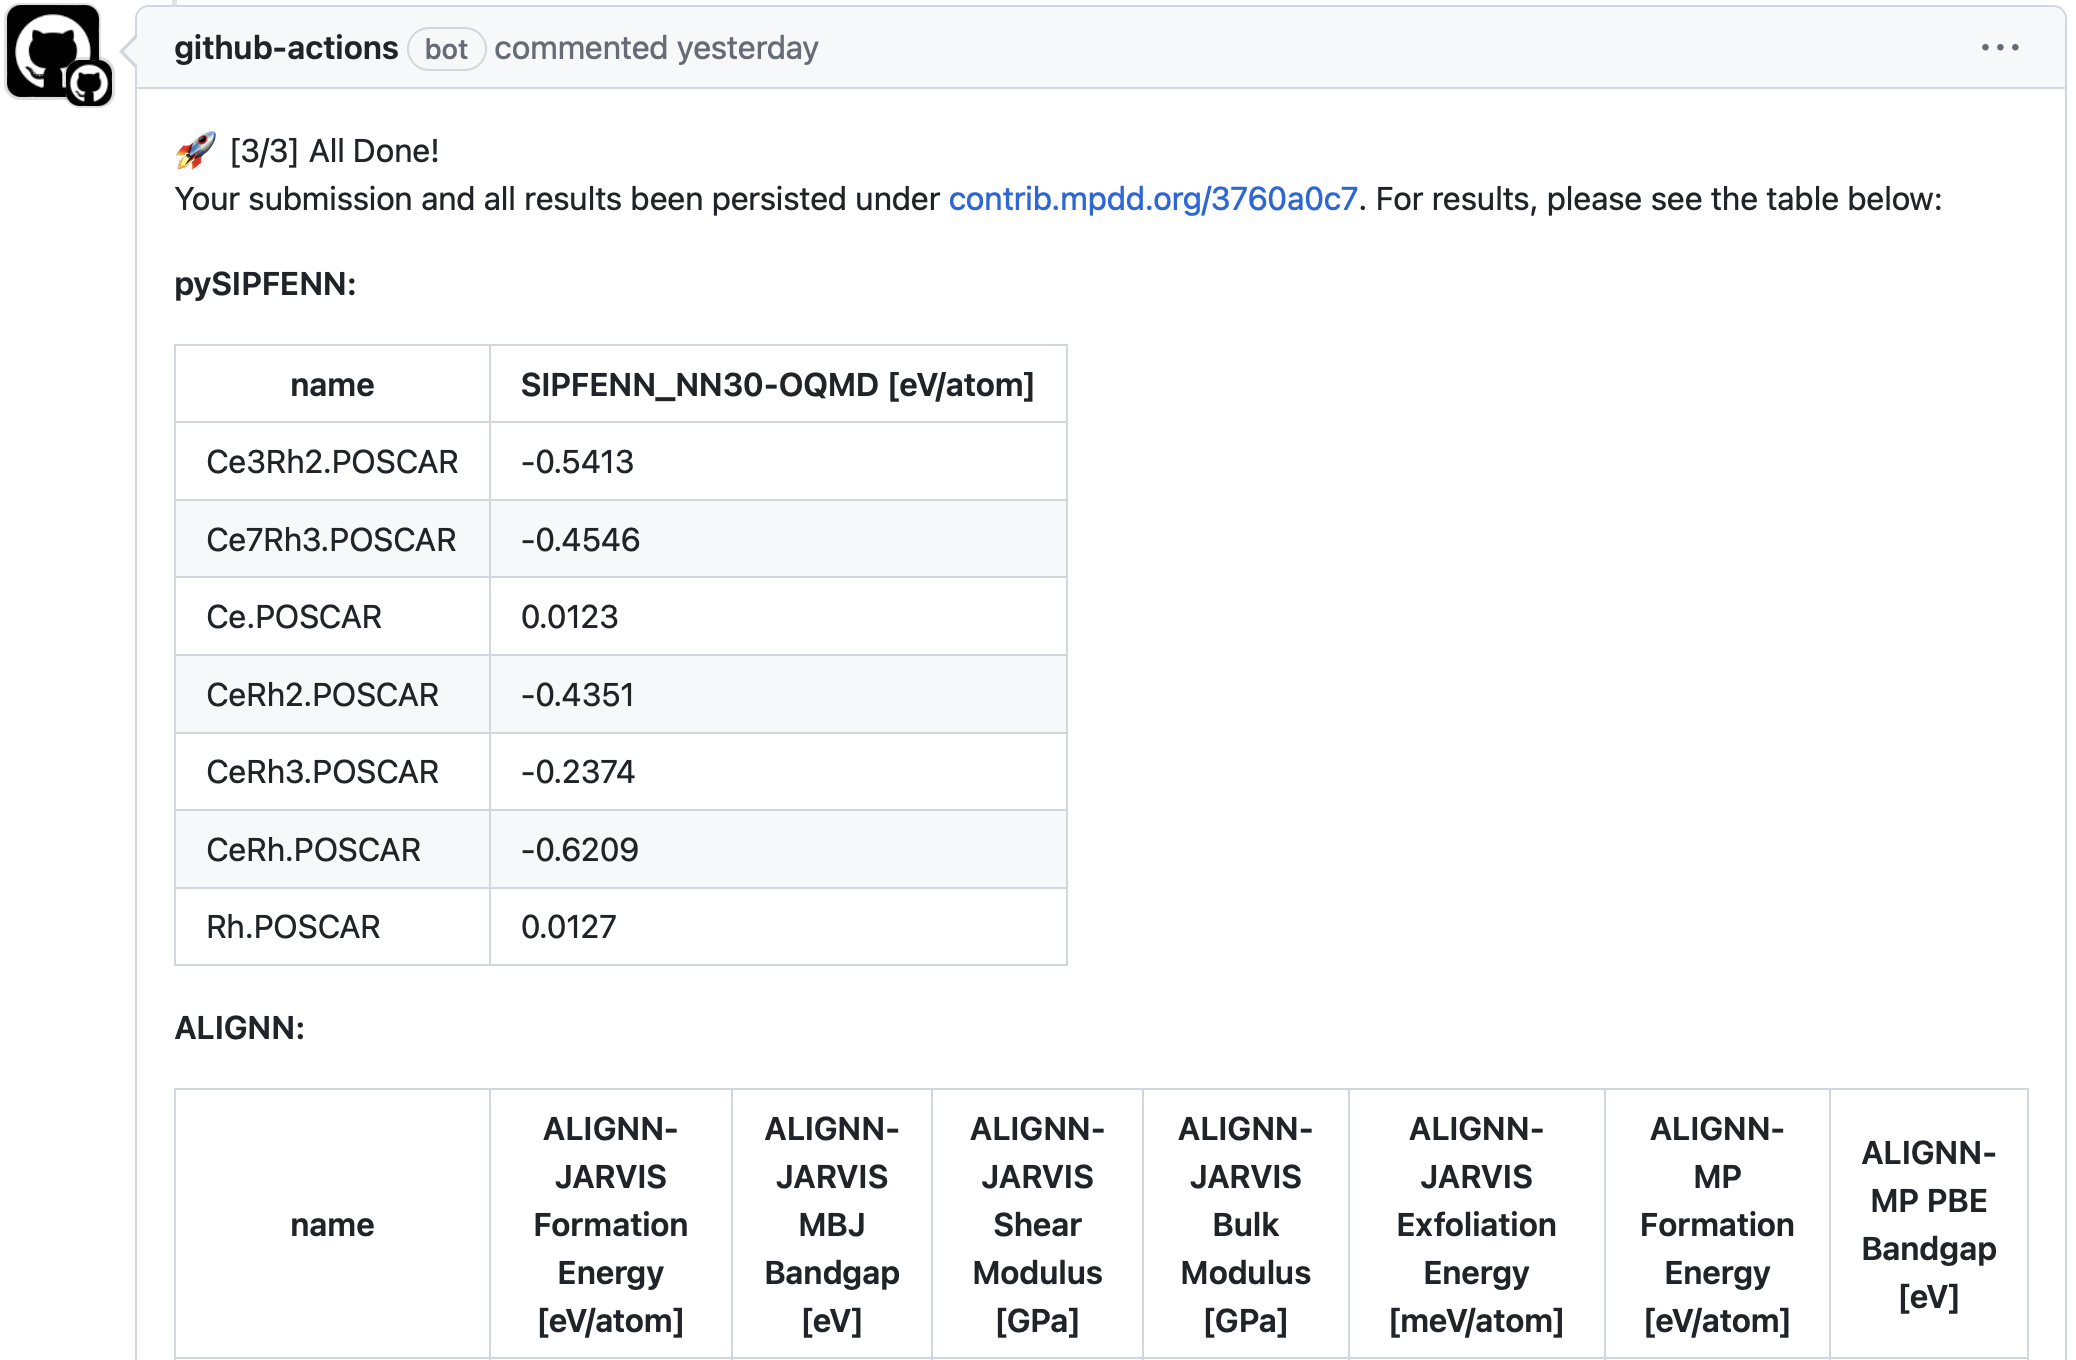
\includegraphics[width=0.8\textwidth]{mpdd/mpddx3.png}
    \caption{Printout of final message after all computation is successfully completed. User is presented with (1) outputs of the ML models deployed on the data and (2) a unique contribution ID based on the commit hash, which can be cited as \texttt{contrib.mpdd.org/3760a0c7} or \texttt{mat-x.org/mpdd-3760a0c7} and points to persisted data record appended with ML results and calculation metadata.}
    \label{mpdd:fig:mpddx3}
\end{figure}

Internally, the contribution is persisted as a commit credited to the submitting user, rather than the computation bot, as shown in Figure~\ref{mpdd:fig:mpddx4}, which consists of a highly-compressed record of the task and its results.

\begin{figure}[H]
    \centering
    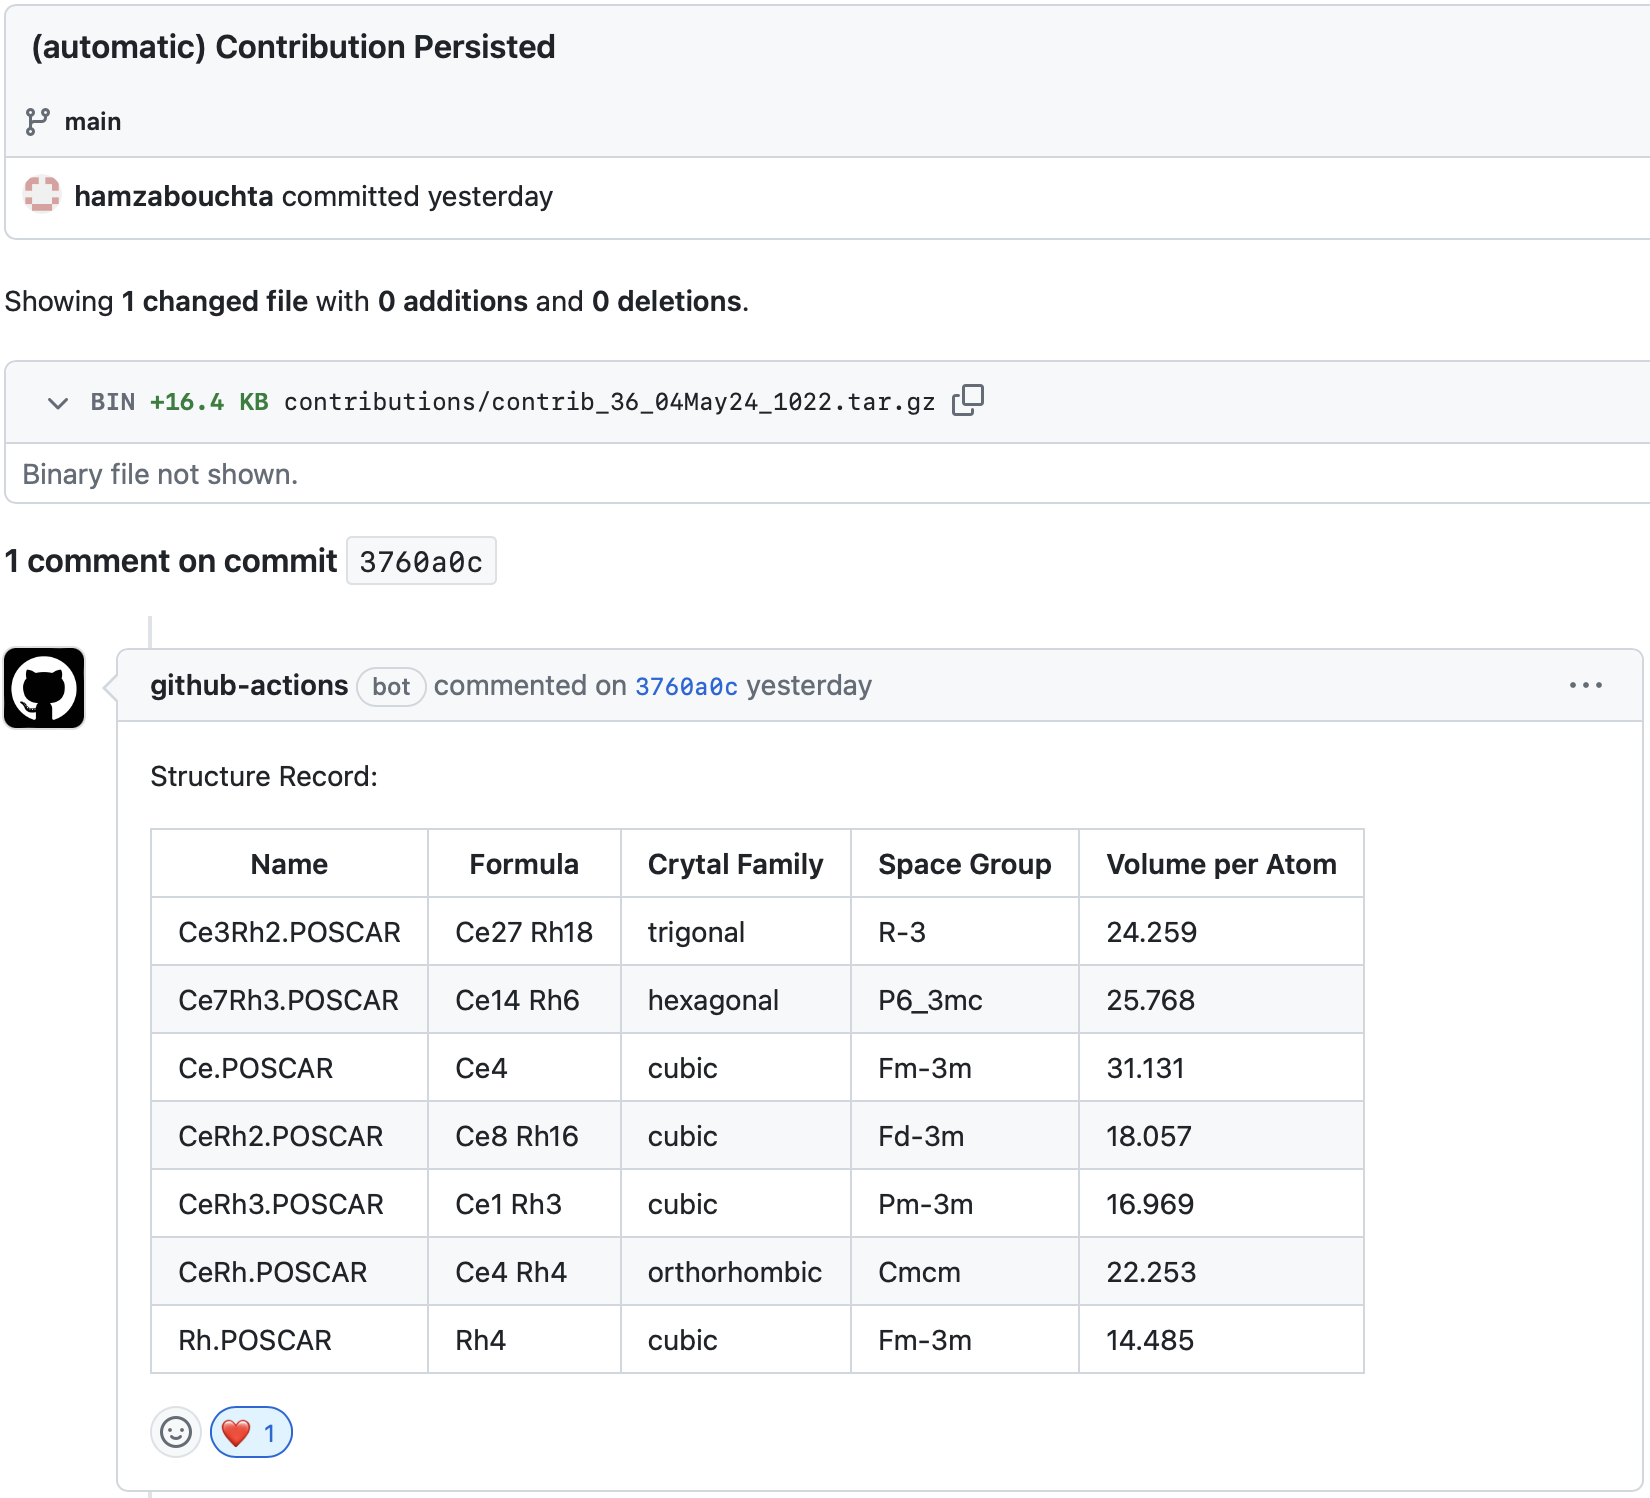
\includegraphics[width=0.85\textwidth]{mpdd/mpddx4.png}
    \caption{Printout of contribution record stored within git repository as auto-generated commit. Right after a successful commit, the system automatically generates a comment on it describing the structures included.}
    \label{mpdd:fig:mpddx4}
\end{figure}

Lastly, at the end of a successful run, the bot comments on the contribution commit with some additional metadata, shown in Figure~\ref{mpdd:fig:mpddx4}, which makes it easier to recognize a particular contribution without its identifier.




\printbibliography[heading=subbibintoc]